\chapter{Problem Analysis}

As discussed in chapter \ref{intro}, uneven module power generation due to mismatches in irradiance, temperature, construction, aging or other factors may lead to inefficient overall power generation. If one of the modules of the PV array is generating below average, it will effect the overall power generation. This situation can be addressed by placing a bypass diode in parallel with every PV panel as shown in figure \ref{BYPASSED_MODULE}. This way the current can flow through the diode, maintaining a higher current in the string. However this solution will drive the power generation in the bypassed module to 0 and will cause a small power loss in the diode. Notice that the total power generated in the string is 120 W instead of 150 W.

\begin{figure}[htbp]
	\begin{center}
		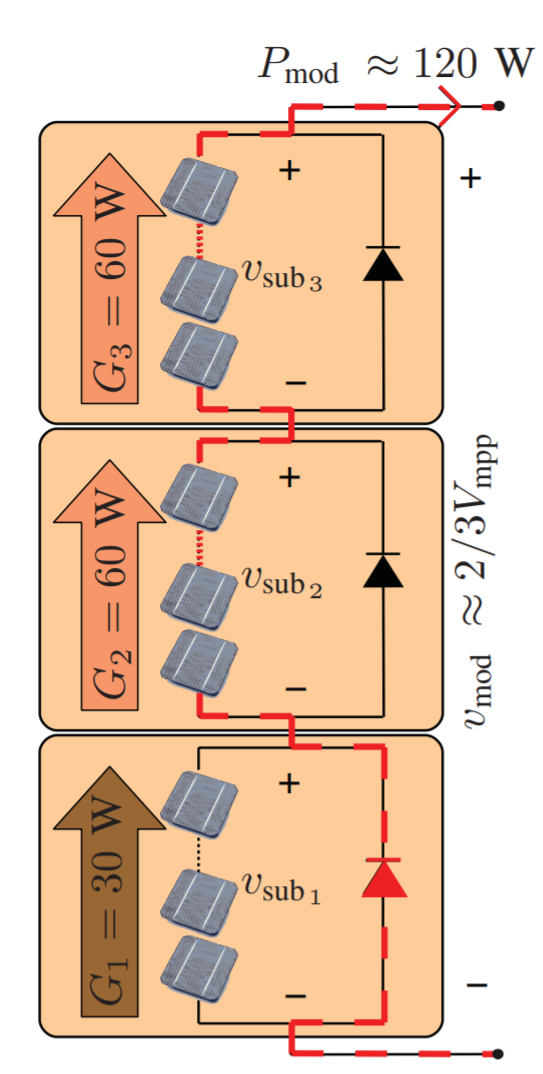
\includegraphics[width=0.3\textwidth]{../Pictures/Uneven_generation}
		\caption{PV module being bypassed by a diode.  %Architectures and Control of Submodule Integrated  DC–DC Converters for Photovoltaic Applications
		}
		\label{BYPASSED_MODULE}
	\end{center}	
\end{figure}

For avoiding the loss of the power generated by the bypassed module, a module integrated converter (MIC) may be used. %[Architectures and Control of Submodule Integrated  DC–DC Converters for Photovoltaic Applications] [Distributed Maximum Power Point Tracking in Photovoltaic Systems – Emerging Architectures and Control Methods] [Submodule Integrated Distributed Maximum Power Point Tracking for Solar Photovoltaic Applications] 
These MICs are usually micro-inverters or DC-DC converters which incorporate a MPPT algorithm in order to maximize the power generated by the module. 
Micro-inverters convert the DC current from the PV directly to grid current. DC-DC converters need an inverter at their output if the desired load is the grid. 
As the micro-inverters have reported higher cost and slightly lower efficiency % [Submodule Integrated Distributed Maximum Power Point Tracking for Solar Photovoltaic Applications] 
the project will be focused in developing a DC-DC MIC for integrating it with a single PV panel.

\section{System requirements}

For the design and test of the MIC it is of great importance to have the requirements of the system defined. The input requirements of the MIC will be based on the specifications of the PV panel \textit{STP300S-24/Vd} from Suntech Power\cite{PV_panel}. 

%\begin{table}[htbp]
%	\centering
%	\begin{tabular}{ |l|c| } 
%		\hline
%		Maximum power ($P_{max}$) & 300 [W]  \\ \hline
%		Optimum Operating Voltage ($V_{mpp}$) & 32.6 [V]  \\ \hline
%		Optimum Operating Current ($I_{mpp}$) & 9.21 [A]  \\ \hline
%		Open Circuit Voltage ($V_{oc}$) &  39.9 [V]\\ \hline
%		Short Circuit Current ($I_{sc}$) & 9.65 [A]  \\ \hline
%		Module Efficiency ($\eta$) & 18.3 \%  \\ \hline
%	\end{tabular}
%	\caption{Electrical characteristics \textit{STP300S-20/Wfb} \cite{PV_panel}.}
%	\label{el_charact_PV_panel}
%\end{table}\todo{I think this table fits better in "Model of the PV panel". Stef}

The specifications of the load of the MIC will be based on the commercial inverter \textit{"Power-one STGU-105"}\cite{power_one_inverter} in order to have the output voltage defined. From the inverter's datasheet it is found that the nominal voltage in the DC-link is 360V, with a maximum input power of 5500W. The development of this project will be based on these requirements because they are real commercial products that the user can purchase. 

The maximum input power, voltage and current of the converter is decided by $P_{max}$, $V_{oc}$ and $I_{sc}$ of the chosen PV-panel. The maximum output voltage is decided by the DC-link voltage and minimum string length, while the minimum output voltage is decided by the maximum string length. The maximum output current is decided by $P_{max}$, which ideally also will be the maximum output power, and the minimum output voltage. Table \ref{MIC_req} shows the requirements of the MIC, extracted from the specifications of the PV panel and the inverter. It defines both the requirements regarding input, output and the length of PV panel strings. 

\begin{table}[H]
	\centering
	\begin{tabular}{|p{6cm}|>{\centering}p{8cm}|}
		\hline
		\rowcolor{lightgray}\multicolumn{2}{|l|}{ \textbf{Input}} \\ \hline
		Maximum input power ($P_{max}$) & 300 [W]  \tabularnewline \hline
		Maximum input Voltage ($V_{oc}$) & 45 [V]  \tabularnewline \hline
		Maximum input current ($I_{sc}$) & 8.67 [A]  \tabularnewline \hline
		
		\rowcolor{lightgray}\multicolumn{2}{|l|}{\textbf{Output}} \tabularnewline \hline
		Maximum output voltage ($V_{out,max}$) & 90 [V] \tabularnewline \hline
		Minimum output voltage ($V_{out,min}$) & 24 [V] \tabularnewline \hline
		Maximum output current ($I_{out,max}$) & 12.5 [A] \tabularnewline \hline
		
		%\rowcolor{lightgray}\multicolumn{2}{|l|}{\textbf{Control}} \tabularnewline \hline
		%Gain margin ($GM$) &  To be defined \tabularnewline \hline
		%Phase margin ($PM$) & To be defined \tabularnewline \hline
		%Rise time ($t_r$) & To be defined \tabularnewline \hline
		%Overshoot ($OS$) & To be defined \tabularnewline \hline
		
		\rowcolor{lightgray}\multicolumn{2}{|l|}{\textbf{PV system specification}} \tabularnewline \hline
		Minimum string length & 4 \tabularnewline \hline
		Maximum string length & 15 \tabularnewline \hline

	\end{tabular}
	\caption{MIC requirements.}
	\label{MIC_req}
\end{table}



%\textbf{Question supervisors:} According to these requirements could we estimate the number of panels to be used? We calculated the necessary duty cycles when working with n panels, and the result can be found in the table below. However we know that when working with duty cycle around 0.75 the currents get quite high, and that depends on the inductance and the switching frequency. Then should we wait until deciding this parameters for deciding the minimum number of panels or should we arbitrarily decide a minimum number of panels and then calculate switching frequency and inductance?

%\begin{table}[H]
%	\centering
%	\begin{tabular}{ |l|c|c|} 
%		\hline
%		Number of PV panels & Buck-boost Duty Cycle & Boost Duty Cycle  \\ \hline
%		1 & 0.91 & 0.91  \\ \hline
%		3 & 0.78 & 0.73 \\ \hline
%		5 &  0.69 & 0.54\\ \hline
%		10 & 0.52 & 0.1  \\ \hline
%	\end{tabular}
%\end{table}

\section{Problem statement}

The problem statement for this project can be formulated as the following question: \newline
\textbf{How can a module integrated converter be designed to maximize the PV power generation under real conditions?}
\newline
\newline
The problem statement will be answered by fulfilling the following objectives: 

\begin{itemize}
	\item Design a DC-DC converter for integration with a PV panel.
	\item Analyze different implementations of MPPT techniques and implement the selected control system. 
	\item Hardware implementation of the MIC components including PCB layout.
	\item Test of the system using a PV simulator and validation of the results. 
\end{itemize}


\section{objectives}